\chapter{Loops and iteration}

Computers are often used to automate repetitive tasks.
Repeating tasks without making errors is something that computers do well and people do poorly.

\index{iteration}

Running the same code multiple times is called {\bf iteration}.
We have seen methods, like \java{countdown} and \java{factorial}, that use recursion to iterate.
Although recursion is elegant and powerful, it takes some getting used to.
Java provides language features that make iteration much easier:
the \java{while} and \java{for} statements.


\section{TODO: String methods}

Most relational operators don't work with strings.
But confusingly, \java{==} and \java{!=} do work with strings -- they just don't do what you expect.
We'll explain what they do later; in the meantime, don't use them with strings.
Instead, you should use the \java{equals} method:

\begin{code}
String fruit1 = "Apple";
String fruit2 = "Orange";
System.out.println(fruit1.equals(fruit2));
\end{code}

The result of \java{fruit1.equals(fruit2)} is the boolean value \java{false}.


\section{The while statement}
\label{while}

\index{while}
\index{loop!while}
\index{statement!while}

Using a \java{while} statement, we can rewrite \java{countdown} like this:

\begin{code}
public static void countdown(int n) {
    while (n > 0) {
        System.out.println(n);
        n = n - 1;
    }
    System.out.println("Blastoff!");
}
\end{code}

You can almost read the \java{while} statement like English:
``While \java{n} is greater than zero, print the value of \java{n} and then reduce the value of \java{n} by 1.
When you get to zero, print Blastoff!''

\index{loop body}

The expression in parentheses is called the condition.
The statements in braces are called the {\bf body}.
The flow of execution for a \java{while} statement is:

\begin{enumerate}

\item Evaluate the condition, yielding \java{true} or \java{false}.

\item If the condition is \java{false}, skip the body and go to the next statement.

\item If the condition is \java{true}, execute the body and go back to step 1.

\end{enumerate}

\index{loop}

This type of flow is called a {\bf loop}, because the last step loops back around to the first.

\index{infinite loop}
\index{loop!infinite}

The body of the loop should change the value of one or more variables so that, eventually, the condition becomes \java{false} and the loop terminates.
Otherwise the loop will repeat forever, which is called an {\bf infinite loop}.
An endless source of amusement for computer scientists is the observation that the directions on shampoo, ``Lather, rinse, repeat,'' are an infinite loop.

In the case of \java{countdown}, we can prove that the loop terminates when \java{n} is positive.
But in general, it is not so easy to tell whether a loop terminates.
For example, this loop continues until \java{n} is 1 (which makes the condition \java{false}):

\begin{code}
public static void sequence(int n) {
    while (n != 1) {
        System.out.println(n);
        if (n % 2 == 0) {         // n is even
            n = n / 2;
        } else {                  // n is odd
            n = n * 3 + 1;
        }
    }
}
\end{code}

Each time through the loop, the program displays the value of \java{n} and then checks whether it is even or odd.
If it is even, the value of \java{n} is divided by two.
If it is odd, the value is replaced by $3n+1$.
For example, if the starting value (the argument passed to \java{sequence}) is 3, the resulting sequence is 3, 10, 5, 16, 8, 4, 2, 1.

Since \java{n} sometimes increases and sometimes decreases, there is no obvious proof that \java{n} will ever reach 1 and that the program will ever terminate.
For some values of \java{n}, we can prove that it terminates.
For example, if the starting value is a power of two, then the value of \java{n} will be even every time through the loop until we get to 1.
The previous example ends with such a sequence, starting when \java{n} is 16.

The hard question is whether this program terminates for {\em all} values of n.
So far, no one has been able to prove it {\em or} disprove it!
For more information, see \url{https://en.wikipedia.org/wiki/Collatz_conjecture}.
%The field of computer science is interested in these types of questions, because their answers give insight to the limits of what computers can and cannot do.


\section{Generating tables}

\index{table}
\index{logarithm}

Loops are good for generating and displaying tabular data.
Before computers were readily available, people had to calculate logarithms, sines and cosines, and other common mathematical functions by hand.
To make that easier, there were books of tables where you could look up values of various functions.
Creating these tables by hand was slow and boring, and the results were often full of errors.

When computers appeared on the scene, one of the initial reactions was: ``This is great!
We can use a computer to generate the tables, so there will be no errors.''
That turned out to be true (mostly), but shortsighted.
Not much later, computers were so pervasive that printed tables became obsolete.

\index{division!floating-point}

Even so, for some operations, computers use tables of values to get an approximate answer, and then perform computations to improve the approximation.
In some cases, there have been errors in the underlying tables, most famously in the table the original Intel Pentium used to perform floating-point division (see \url{https://en.wikipedia.org/wiki/Pentium_FDIV_bug}).

Although a ``log table'' is not as useful as it once was, it still makes a good example of iteration.
The following loop displays a table with a sequence of values in the left column and their logarithms in the right column:

\begin{code}
int i = 1;
while (i < 10) {
    double x = i;
    System.out.println(x + "   " + Math.log(x));
    i = i + 1;
}
\end{code}

The output of this program is:

\begin{stdout}
1.0   0.0
2.0   0.6931471805599453
3.0   1.0986122886681098
4.0   1.3862943611198906
5.0   1.6094379124341003
6.0   1.791759469228055
7.0   1.9459101490553132
8.0   2.0794415416798357
9.0   2.1972245773362196
\end{stdout}

\java{Math.log} computes natural logarithms, that is, logarithms base $e$.
For computer science applications, we often want logarithms with respect to base 2.
To compute them, we can apply this equation:
%
\[ \log_2 x = \frac{log_e x}{log_e 2} \]
%
We can modify the loop as follows:

\begin{code}
int i = 1;
while (i < 10) {
    double x = i;
    System.out.println(x + "   " + Math.log(x) / Math.log(2));
    i = i + 1;
}
\end{code}

And here are the results:

\begin{stdout}
1.0   0.0
2.0   1.0
3.0   1.5849625007211563
4.0   2.0
5.0   2.321928094887362
6.0   2.584962500721156
7.0   2.807354922057604
8.0   3.0
9.0   3.1699250014423126
\end{stdout}

Each time through the loop, we add one to \java{x}, so the result is an arithmetic sequence.
If we multiply \java{x} by something instead, we get a geometric sequence:

\begin{code}
final double LOG2 = Math.log(2);
int i = 1;
while (i < 100) {
    double x = i;
    System.out.println(x + "   " + Math.log(x) / LOG2);
    i = i * 2;
}
\end{code}

\index{final}

The first line stores \java{Math.log(2)} in a \java{final} variable to avoid computing that value over and over again.
The last line multiplies \java{x} by 2.
The result is:

\begin{stdout}
1.0   0.0
2.0   1.0
4.0   2.0
8.0   3.0
16.0   4.0
32.0   5.0
64.0   6.0
\end{stdout}

This table shows the powers of two and their logarithms, base 2.
Log tables may not be useful anymore, but for computer scientists, knowing the powers of two helps a lot!
%When you have an idle moment, you should memorize the powers of two up to 65536 (that's $2^{16}$).


\section{Encapsulation and generalization}
\label{encapsulation}

\index{table!two-dimensional}
\index{program development}

In Section~\ref{distance}, we presented a way of writing programs called incremental development.
In this section we present another {\bf program development} process called ``encapsulation and generalization''.
The steps are:

\begin{enumerate}

\item Write a few lines of code in \java{main} or another method, and test them.

\item When they are working, wrap them in a new method, and test again.

\item If it's appropriate, replace literal values with variables and parameters.

\end{enumerate}

\index{encapsulate}
\index{generalize}

The second step is called {\bf encapsulation}; the third step is {\bf generalization}.

To demonstrate this process, we'll develop methods that display multiplication tables.
Here is a loop that displays the multiples of two, all on one line:

\begin{code}
int i = 1;
while (i <= 6) {
    System.out.printf("%4d", 2 * i);
    i = i + 1;
}
System.out.println();
\end{code}

\index{loop variable}
\index{variable!loop}

The first line initializes a variable named \java{i}, which is going to act as a {\bf loop variable}: as the loop executes, the value of \java{i} increases from 1 to 6; when \java{i} is 7, the loop terminates.

Each time through the loop, we display the value \java{2 * i} padded with spaces so it's four characters wide.
Since we use \java{System.out.printf}, the output appears on a single line.

After the loop, we call \java{println} to print a newline and complete the line.
Remember that in some environments, none of the output is displayed until the line is complete.

The output of the code so far is:

\begin{stdout}
   2   4   6   8  10  12
\end{stdout}

The next step is to ``encapsulate'' this code in a new method.
Here's what it looks like:

\begin{code}
public static void printRow() {
    int i = 1;
    while (i <= 6) {
        System.out.printf("%4d", 2 * i);
        i = i + 1;
    }
    System.out.println();
}
\end{code}

\index{generalization}

Next we replace the constant value, \java{2}, with a parameter, \java{n}.
This step is called ``generalization'' because it makes the method more general (less specific).

\begin{code}
public static void printRow(int n) {
    int i = 1;
    while (i <= 6) {
        System.out.printf("%4d", n * i);
        i = i + 1;
    }
    System.out.println();
}
\end{code}

Invoking this method with the argument 2 yields the same output as before.
With the argument 3, the output is:

\begin{stdout}
   3   6   9  12  15  18
\end{stdout}

And with argument 4, the output is:

\begin{stdout}
   4   8  12  16  20  24
\end{stdout}

By now you can probably guess how we are going to display a multiplication table: we'll invoke \java{printRow} repeatedly with different arguments.
In fact, we'll use another loop to iterate through the rows.

\begin{code}
int i = 1;
while (i <= 6) {
    printRow(i);
    i = i + 1;
}
\end{code}

And the output looks like this:

\begin{stdout}
   1   2   3   4   5   6
   2   4   6   8  10  12
   3   6   9  12  15  18
   4   8  12  16  20  24
   5  10  15  20  25  30
   6  12  18  24  30  36
\end{stdout}

The format specifier \java{\%4d} in \java{printRow} causes the output to align vertically, regardless of whether the numbers are one or two digits.

Finally, we encapsulate the second loop in a method:

\begin{code}
public static void printTable() {
    int i = 1;
    while (i <= 6) {
        printRow(i);
        i = i + 1;
    }
}
\end{code}

One of the challenges of programming, especially for beginners, is figuring out how to divide up a program into methods.
The process of encapsulation and generalization allows you to design as you go along.


\section{More generalization}

\index{generalization}

The previous version of \java{printTable} always displays six rows.
We can generalize it by replacing the literal \java{6} with a parameter:

\begin{code}
public static void printTable(int rows) {
    int i = 1;
    while (i <= rows) {
        printRow(i);
        i = i + 1;
    }
}
\end{code}

Here is the output with the argument 7:

\begin{stdout}
   1   2   3   4   5   6
   2   4   6   8  10  12
   3   6   9  12  15  18
   4   8  12  16  20  24
   5  10  15  20  25  30
   6  12  18  24  30  36
   7  14  21  28  35  42
\end{stdout}

That's better, but it still has a problem: it always displays the same number of columns.
We can generalize more by adding a parameter to \java{printRow}:

\begin{code}
public static void printRow(int n, int cols) {
    int i = 1;
    while (i <= cols) {
        System.out.printf("%4d", n * i);
        i = i + 1;
    }
    System.out.println();
}
\end{code}

Now \java{printRow} takes two parameters: \java{n} is the value whose multiples should be displayed, and \java{cols} is the number of columns.
Since we added a parameter to \java{printRow}, we also have to change the line in \java{printTable} where it is invoked:

\begin{code}
public static void printTable(int rows) {
    int i = 1;
    while (i <= rows) {
        printRow(i, rows);
        i = i + 1;
    }
}
\end{code}

When this line executes, it evaluates \java{rows} and passes the value, which is 7 in this example, as an argument.
In \java{printRow}, this value is assigned to \java{cols}.
As a result, the number of columns equals the number of rows, so we get a square 7x7 table:

\begin{stdout}
   1   2   3   4   5   6   7
   2   4   6   8  10  12  14
   3   6   9  12  15  18  21
   4   8  12  16  20  24  28
   5  10  15  20  25  30  35
   6  12  18  24  30  36  42
   7  14  21  28  35  42  49
\end{stdout}

When you generalize a method appropriately, you often find that it has capabilities you did not plan.
For example, you might notice that the multiplication table is symmetric; since $ab = ba$, all the entries in the table appear twice.
You could save ink by printing half of the table, and you would only have to change one line of \java{printTable}:

\begin{code}
printRow(i, i);
\end{code}

In words, the length of each row is the same as its row number.
The result is a triangular multiplication table.

\begin{stdout}
   1
   2   4
   3   6   9
   4   8  12  16
   5  10  15  20  25
   6  12  18  24  30  36
   7  14  21  28  35  42  49
\end{stdout}

Generalization makes code more versatile, more likely to be reused, and sometimes easier to write.

%Even though the second parameter in \java{printRow} is named \java{size} and we have a variable with the same name, we can still use any value or expression we want for the argument.

%Remember, you do not pass {\em variables} to methods; you pass their current {\em values}.
%In this last example, the value of \java{i} in \java{printTable} is assigned to both \java{n} and \java{cols} in \java{printRow}.


\section{The for statement}
\label{for}

\index{for}
\index{loop!for}
\index{statement!for}

The loops we have written so far have several elements in common.
They start by initializing a variable, they have a condition that depends on that variable, and inside the loop they do something to update that variable.
This type of loop is so common that there is another statement, the \java{for} loop, that expresses it more concisely.

For example, we could rewrite \java{printTable} like this:

\begin{code}
public static void printTable(int rows) {
    for (int i = 1; i <= rows; i = i + 1) {
        printRow(i, rows);
    }
}
\end{code}

\java{for} loops have three components in parentheses, separated by semicolons: the initializer, the condition, and the update.

\begin{enumerate}

\item The {\em initializer} runs once at the very beginning of the loop.

\item The {\em condition} is checked each time through the loop.
If it is \java{false}, the loop ends.
Otherwise, the body of the loop is executed (again).

\item At the end of each iteration, the {\em update} runs, and we go back to step 2.

\end{enumerate}

The \java{for} loop is often easier to read because it puts all the loop-related statements at the top of the loop.

There is one difference between \java{for} loops and \java{while} loops: if you declare a variable in the initializer, it only exists inside the \java{for} loop.
For example, here is a version of \java{printRow} that uses a \java{for} loop:

\begin{code}
public static void printRow(int n, int cols) {
    for (int i = 1; i <= cols; i = i + 1) {
        System.out.printf("%4d", n * i);
    }
    System.out.println(i);  // compiler error
}
\end{code}

The last line tries to display \java{i} (for no reason other than demonstration) but it won't work.
If you need to use a loop variable outside the loop, you have to declare it outside the loop, like this:

\begin{code}
public static void printRow(int n, int cols) {
    int i;
    for (i = 1; i <= cols; i = i + 1) {
        System.out.printf("%4d", n * i);
    }
    System.out.println(i);
}
\end{code}

\index{increment}
\index{decrement}

Assignments like \java{i = i + 1} don't often appear in \java{for} loops, because Java provides a more concise way to add and subtract by one.
Specifically, \java{++} is the {\bf increment} operator; it has the same effect as \java{i = i + 1}.
And \java{--} is the {\bf decrement} operator; it has the same effect as \java{i = i - 1}.

If you want to increment or decrement a variable by an amount other than \java{1}, you can use \java{+=} and \java{-=}.
For example, \java{i += 2} increments \java{i} by \java{2}.


\section{The do-while loop}

\index{pretest loop}

The \java{while} and \java{for} statements are {\bf pretest loops}; that is, they test the condition first and at the beginning of each pass through the loop.

\index{posttest loop}
\index{do-while}

Java also provides a {\bf posttest loop}: the \java{do}-\java{while} statement.
This type of loop is useful when you need to run the body of the loop at least once.

%NOTE: can we find an example that's better using do-while than using while-break?

For example, in Section~\ref{validate} we used the \java{return} statement to avoid reading invalid input from the user.
We can use a \java{do}-\java{while} loop to keep reading input until it's valid:

\begin{code}
Scanner in = new Scanner(System.in);
boolean okay;
do {
    System.out.print("Enter a number: ");
    if (in.hasNextDouble()) {
        okay = true;
    } else {
        okay = false;
        String word = in.next();
        System.err.println(word + " is not a number");
    }
} while (!okay);
double x = in.nextDouble();
\end{code}

Although this code looks complicated, it is essentially only three steps:

\begin{enumerate}
\item Display a prompt.
\item Check the input; if invalid, display an error and start over.
\item Read the input.
\end{enumerate}

\index{System.err}

The code uses a flag variable, \java{okay}, to indicate whether we need to repeat the loop body.
If \java{hasNextDouble()} returns \java{false}, we consume the invalid input by calling \java{next()}.
We then display an error message via \java{System.err}.
The loop terminates when \java{hasNextDouble()} return \java{true}.


\section{Break and continue}

Sometimes neither a pretest nor a posttest loop will provide exactly what you need.
In the previous example, the ``test'' needed to happen in the middle of the loop.
As a result, we used a flag variable and a nested \java{if}-\java{else} statement.

\index{break}

A simpler way to solve this problem is to use a \java{break} statement.
When a program reaches a \java{break} statement, it exits the current loop.

\begin{code}
Scanner in = new Scanner(System.in);
while (true) {
    System.out.print("Enter a number: ");
    if (in.hasNextDouble()) {
        break;
    }
    String word = in.next();
    System.err.println(word + " is not a number");
}
double x = in.nextDouble();
\end{code}

Using \java{true} as a conditional in a \java{while} loop is an idiom that means ``loop forever'', or in this case ``loop until you get to a \java{break} statement.''

\index{continue}

In addition to the \java{break} statement, which exits the loop, Java provides a \java{continue} statement that moves on to the next iteration.
For example, the following code reads integers from the keyboard and computes a running total.
The \java{continue} statement causes the program to skip over any negative values.

\begin{code}
Scanner in = new Scanner(System.in);
int x = -1;
int sum = 0;
while (x != 0) {
    x = in.nextInt();
    if (x <= 0) {
        continue;
    }
    System.out.println("Adding " + x);
    sum += x;
}
\end{code}

Although \java{break} and \java{continue} statements give you more control of the loop execution, they can make code difficult to understand and debug.
Use them sparingly.


\section{Reading documentation}
\label{sec:apidocs}

\index{documentation}

One of the nice things about Java is that it comes with an extensive library of classes and methods.
But before you use them, you might have to read the documentation.
And sometimes that's not easy.

As an example, let's look at the documentation for \java{Scanner}, which we used in Section~\ref{scanner}.
You can find it by doing a web search for ``Java Scanner''.
Figure~\ref{fig.scanner} shows a screenshot of the page.

\begin{figure}[!ht]
\begin{center}
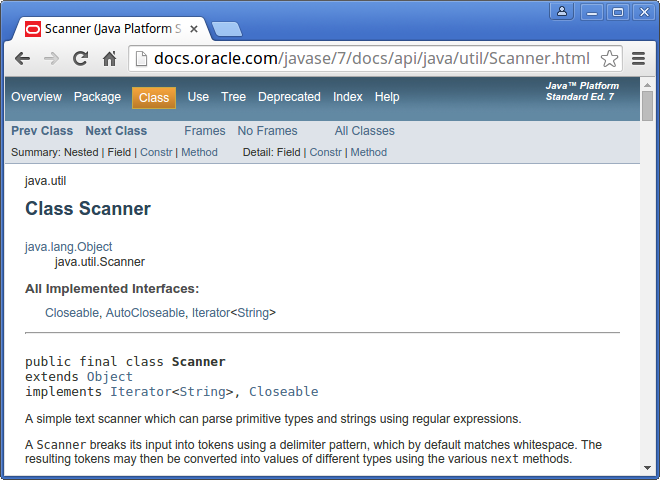
\includegraphics[width=0.9\textwidth]{figs/scanner.png}
\caption{Screenshot of the documentation for \java{Scanner}.}
\label{fig.scanner}
\end{center}
\end{figure}

Documentation for other classes uses a similar format.
The first line is the package that contains the class, such as \java{java.util}.
The second line is the name of the class.
The ``Implemented Interfaces'' section lists some of the things a \java{Scanner} can do; we won't say more about that for now.

%The next two lines indicate that every \java{Scanner} is also an \java{Object}; that will make more sense after Section~\ref{inheritance}.

The next section of the documentation is a narrative that explains the purpose of the class and includes examples of how to use it.
This text can be difficult to read because it uses terms we have not learned yet.
But the examples are often very useful.
A good way to get started with a new class is to paste the examples into a test file and see if you can compile and run them.

One of the examples shows how you can use a \java{Scanner} to read input from a \java{String} instead of \java{System.in}:

%NOTE: only use of Scanner w/o System.in; mention this again in String chapter?
\begin{code}
String input = "1 fish 2 fish red fish blue fish";
Scanner s = new Scanner(input);
\end{code}

After the narrative, code examples, and some other details, you will find the following tables:

\begin{description}

\item[Constructor summary:]
Ways of creating, or ``constructing'', a \java{Scanner}.

\item[Method summary:]
The list of methods that \java{Scanner} provides.

\item[Constructor detail:]
More information about how to create a \java{Scanner}.

\item[Method detail:]
More information about each method.

\end{description}

As an example, here is the summary information for \java{nextInt}:

\begin{stdout}
public int nextInt()
Scans the next token of the input as an int.
\end{stdout}

\index{signature}

The first line is the method's {\bf signature}, which specifies the name of the method, its parameters (none), and what type it returns (\java{int}).
The next line is a short description of what it does.

The ``Method detail'' explains more:

\begin{stdout}
public int nextInt()
Scans the next token of the input as an int.

An invocation of this method of the form nextInt() behaves in
exactly the same way as the invocation nextInt(radix), where
radix is the default radix of this scanner.

Returns:
the int scanned from the input

Throws:
InputMismatchException - if the next token does not match
    the Integer regular expression, or is out of range
NoSuchElementException - if input is exhausted
IllegalStateException - if this scanner is closed
\end{stdout}

The ``Returns'' section describes the result when the method succeeds.
In contrast, the ``Throws'' section describes possible errors and their resulting exceptions.
Exceptions are said to be ``thrown'', like a referee throwing a flag, or like a toddler throwing a fit.

It might take you some time to get comfortable reading documentation and learning which parts to ignore.
But it's worth the effort.
Knowing what's available in the library helps you avoid reinventing the wheel.
And a little bit of documentation can save you a lot of debugging.


\section{Writing documentation}
\label{sec:javadoc}

As you benefit from reading good documentation, you should ``pay it forward'' by writing good documentation.
A nice feature of the Java language is the ability to embed documentation in your source code.
That way, you can write it as you go, and as things change, it is easier to keep the documentation consistent with the code.

\index{HTML}
\index{Javadoc}

If you include documentation in your source code, you can extract it automatically, and generate well-formatted HTML, using a tool called {\bf Javadoc}.
This tool is included in standard Java development environments, and it is widely used.
In fact, the online documentation of the Java libraries is generated by Javadoc.

\index{comment!documentation}
\index{documentation!Javadoc comments}

Javadoc scans your source files looking for specially-formatted {\bf documentation comments}, also known as ``Javadoc comments''.
They begin with \java{/**} (two stars) and end with \java{*/} (one star).
Anything in between is considered part of the documentation.

Here's a class definition with two Javadoc comments, one for the class and one for the \java{main} method:

\begin{code}
/**
 * Example program that demonstrates print vs println.
 */
public class Goodbye {

    /**
     * Prints a greeting.
     */
    public static void main(String[] args) {
        System.out.print("Goodbye, ");  // note the space
        System.out.println("cruel world");
    }
}
\end{code}

The class comment explains the purpose of the class.
The method comment explains what the method does.

Notice that this example also includes an inline comment, beginning with \java{//}.
In general, inline comments are short phrases that help explain complex parts of a program.
They are intended for other programmers reading and maintaining the source code.

In contrast, Javadoc comments are longer, usually complete sentences.
They explain what each method does, but they omit details about how the method works.
And they are intended for people who will use the methods without looking at the source code.

Appropriate comments and documentation are essential for making source code readable.
And remember that the person most likely to read your code in the future, and appreciate good documentation, is you.


\section{Javadoc tags}

In Section~\ref{sec:javadoc}, we discussed how to write documentation comments using \java{/**}.
It's generally a good idea to document each class and method, so that other programmers can understand what they do without having to read the code.

\index{tag}
\index{param tag}
\index{return tag}
\index{documentation!Javadoc tags}

To organize the documentation into sections, Javadoc supports optional {\bf tags} that begin with the at sign (\java{@}).
For example, we can use \java{@param} and \java{@return} to provide additional information about parameters and return values.

\begin{code}
/**
 * Tests whether x is a single digit integer.
 *
 * @param x the integer to test
 * @return true if x has one digit, false otherwise
 */
public static boolean isSingleDigit(int x) {
\end{code}

\index{HTML}
\index{Javadoc}

Figure~\ref{fig.javadoc} shows part of the resulting HTML page generated by Javadoc.
Notice the relationship between the source code and the documentation.

\begin{figure}[!ht]
\begin{center}
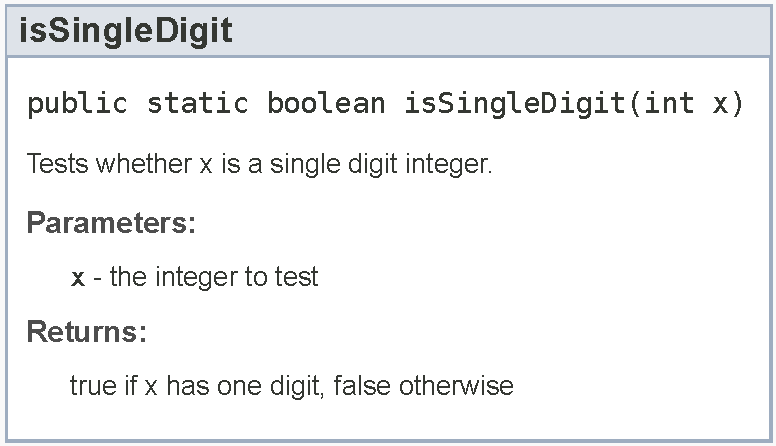
\includegraphics[scale=0.8]{figs/javadoc.pdf}
\caption{HTML documentation for \java{isSingleDigit}.}
\label{fig.javadoc}
\end{center}
\end{figure}

Methods with multiple parameters should have separate \java{@param} tags that describe each one.
Void methods should have no \java{@return} tag, since they do not return a value.


\section{Vocabulary}

\begin{description}

\term{iteration}
Executing a sequence of statements repeatedly.

\term{loop}
A statement that executes a sequence of statements repeatedly.

\term{loop body}
The statements inside the loop.

\term{infinite loop}
A loop whose condition is always true.

\term{program development}
A process for writing programs.
So far we have seen ``incremental development'' and ``encapsulation and generalization''.

\term{encapsulate}
To wrap a sequence of statements in a method.

\term{generalize}
To replace something unnecessarily specific (like a constant value) with something appropriately general (like a variable or parameter).

\term{loop variable}
A variable that is initialized, tested, and updated in order to control a loop.

\term{increment}
Increase the value of a variable.

\term{decrement}
Decrease the value of a variable.

\term{pretest loop}
A loop that tests the condition before each iteration.

\term{posttest loop}
A loop that tests the condition after each iteration.

\end{description}


\section{Exercises}

The code for this chapter is in the {\tt ch06} directory of {\tt ThinkJava2Code}.
See page~\pageref{code} for instructions on how to download the repository.
Before you start the exercises, we recommend that you compile and run the examples.

If you have not already read Appendix~\ref{checkstyle}, now might be a good time.
It describes Checkstyle, a tool that analyzes many aspects of your source code.


\begin{exercise}

Consider the following methods:

\begin{code}
public static void main(String[] args) {
    loop(10);
}

public static void loop(int n) {
    int i = n;
    while (i > 1) {
        System.out.println(i);
        if (i % 2 == 0) {
            i = i / 2;
        } else {
            i = i + 1;
        }
    }
}
\end{code}

\begin{enumerate}

\item Draw a table that shows the value of the variables \java{i} and \java{n} during the execution of \java{loop}.
The table should contain one column for each variable and one line for each iteration.

\item What is the output of this program?

\item Can you prove that this loop terminates for any positive value of \java{n}?

% If i is odd and we increment by 1, the result is even.  So the second
% branch is always followed by the first branch.
% If i is even and we divide by 2, the result might be odd.  So in the
% worst case, we might alternate between the branches.
% But we can't do more of the second branch than the first.
% So we divide at least as often as we add.

% If i is 1, we're done.
% If i is 2, we divide by 2 and we're done.
% If i is greater than 2, the first branch decreases more than the
% second branch increases.
% So if we do one of each, the net effect is a decrease.
% Therefore, the value of i has to decrease after any two steps.

\end{enumerate}

\end{exercise}


\begin{exercise}

Let's say you are given a number, $a$, and you want to find its square root.
One way to do that is to start with a rough guess about the answer, $x_0$, and then improve the guess using this formula:
%
\[ x_1 =(x_0 + a/x_0) / 2 \]
%
For example, if we want to find the square root of 9, and we start with $x_0 = 6$, then $x_1 = (6 + 9/6) / 2 = 3.75$, which is closer.
We can repeat the procedure, using $x_1$ to calculate $x_2$, and so on.
In this case, $x_2 = 3.075$ and $x_3 = 3.00091$.
So it converges quickly on the correct answer.

Write a method called \java{squareRoot} that takes a \java{double} and returns an approximation of the square root of the parameter, using this technique.
You should not use \java{Math.sqrt}.

As your initial guess, you should use $a/2$.
Your method should iterate until it gets two consecutive estimates that differ by less than 0.0001.
%In other words, return when the absolute value of $x_n - x_{n-1}$ is less than 0.0001.
You can use \java{Math.abs} to calculate the absolute value of the difference.

\end{exercise}


\begin{exercise}

In Exercise~\ref{ex.power} we wrote a recursive version of \java{power}, which takes a double \java{x} and an integer \java{n} and returns $x^n$.
Now write an iterative method to perform the same calculation.

\end{exercise}


\begin{exercise}

Section~\ref{factorial} presents a recursive method that computes the factorial function.
Write an iterative version of \java{factorial}.

\end{exercise}


\begin{exercise}

One way to calculate $e^x$ is to use the infinite series expansion:
%
\[ e^x = 1 + x + x^2 / 2! + x^3 / 3! + x^4 / 4! + \ldots \]
%
The $i$th term in the series is $x^i / i!$.

\begin{enumerate}

\item Write a method called \java{myexp} that takes \java{x} and \java{n} as parameters and estimates $e^x$ by adding the first \java{n} terms of this series.
You can use the \java{factorial} method from Section~\ref{factorial} or your iterative version from the previous exercise.

\index{efficiency}

\item You can make this method more efficient if you realize that the numerator of each term is the same as its predecessor multiplied by \java{x}, and the denominator is the same as its predecessor multiplied by \java{i}.
Use this observation to eliminate the use of \java{Math.pow} and \java{factorial}, and check that you get the same result.

\item Write a method called \java{check} that takes a parameter, \java{x}, and displays \java{x}, \java{myexp(x)}, and \java{Math.exp(x)}.
The output should look something like:

\begin{stdout}
1.0     2.708333333333333     2.718281828459045
\end{stdout}

You can use the escape sequence \java{"\\t"} to put a tab character between columns of a table.

\item Vary the number of terms in the series (the second argument that \java{check} sends to \java{myexp}) and see the effect on the accuracy of the result.
Adjust this value until the estimated value agrees with the correct answer when \java{x} is 1.

\item Write a loop in \java{main} that invokes \java{check} with the values 0.1, 1.0, 10.0, and 100.0.
How does the accuracy of the result vary as \java{x} varies?
Compare the number of digits of agreement rather than the difference between the actual and estimated values.

\item Add a loop in \java{main} that checks \java{myexp} with the values -0.1, -1.0, -10.0, and -100.0.
Comment on the accuracy.

\end{enumerate}

\end{exercise}


\begin{exercise}

One way to evaluate $\exp(-x^2)$ is to use the infinite series expansion:
%
\[ \exp(-x^2) = 1 - x^2 + x^4/2 - x^6/6 + \ldots \]
%
The $i$th term in this series is $(-1)^i x^{2i} / i!$.
Write a method named \java{gauss} that takes \java{x} and \java{n} as arguments and returns the sum of the first \java{n} terms of the series.
You should not use \java{factorial} or \java{pow}.

\end{exercise}
